% Options for packages loaded elsewhere
\PassOptionsToPackage{unicode}{hyperref}
\PassOptionsToPackage{hyphens}{url}
%
\documentclass[
  12pt,
]{article}
\usepackage{amsmath,amssymb}
\usepackage[]{mathpazo}
\usepackage{iftex}
\ifPDFTeX
  \usepackage[T1]{fontenc}
  \usepackage[utf8]{inputenc}
  \usepackage{textcomp} % provide euro and other symbols
\else % if luatex or xetex
  \usepackage{unicode-math}
  \defaultfontfeatures{Scale=MatchLowercase}
  \defaultfontfeatures[\rmfamily]{Ligatures=TeX,Scale=1}
\fi
% Use upquote if available, for straight quotes in verbatim environments
\IfFileExists{upquote.sty}{\usepackage{upquote}}{}
\IfFileExists{microtype.sty}{% use microtype if available
  \usepackage[]{microtype}
  \UseMicrotypeSet[protrusion]{basicmath} % disable protrusion for tt fonts
}{}
\makeatletter
\@ifundefined{KOMAClassName}{% if non-KOMA class
  \IfFileExists{parskip.sty}{%
    \usepackage{parskip}
  }{% else
    \setlength{\parindent}{0pt}
    \setlength{\parskip}{6pt plus 2pt minus 1pt}}
}{% if KOMA class
  \KOMAoptions{parskip=half}}
\makeatother
\usepackage{xcolor}
\IfFileExists{xurl.sty}{\usepackage{xurl}}{} % add URL line breaks if available
\IfFileExists{bookmark.sty}{\usepackage{bookmark}}{\usepackage{hyperref}}
\hypersetup{
  pdftitle={FB Analysis},
  pdfauthor={Kim, Brew, Zilinsky},
  hidelinks,
  pdfcreator={LaTeX via pandoc}}
\urlstyle{same} % disable monospaced font for URLs
\usepackage[margin=1in]{geometry}
\usepackage{longtable,booktabs,array}
\usepackage{calc} % for calculating minipage widths
% Correct order of tables after \paragraph or \subparagraph
\usepackage{etoolbox}
\makeatletter
\patchcmd\longtable{\par}{\if@noskipsec\mbox{}\fi\par}{}{}
\makeatother
% Allow footnotes in longtable head/foot
\IfFileExists{footnotehyper.sty}{\usepackage{footnotehyper}}{\usepackage{footnote}}
\makesavenoteenv{longtable}
\usepackage{graphicx}
\makeatletter
\def\maxwidth{\ifdim\Gin@nat@width>\linewidth\linewidth\else\Gin@nat@width\fi}
\def\maxheight{\ifdim\Gin@nat@height>\textheight\textheight\else\Gin@nat@height\fi}
\makeatother
% Scale images if necessary, so that they will not overflow the page
% margins by default, and it is still possible to overwrite the defaults
% using explicit options in \includegraphics[width, height, ...]{}
\setkeys{Gin}{width=\maxwidth,height=\maxheight,keepaspectratio}
% Set default figure placement to htbp
\makeatletter
\def\fps@figure{htbp}
\makeatother
\setlength{\emergencystretch}{3em} % prevent overfull lines
\providecommand{\tightlist}{%
  \setlength{\itemsep}{0pt}\setlength{\parskip}{0pt}}
\setcounter{secnumdepth}{-\maxdimen} % remove section numbering
\usepackage{booktabs}
\usepackage{longtable}
\usepackage{array}
\usepackage{multirow}
\usepackage{wrapfig}
\usepackage{float}
\usepackage{colortbl}
\usepackage{pdflscape}
\usepackage{tabu}
\usepackage{threeparttable}
\usepackage{threeparttablex}
\usepackage[normalem]{ulem}
\usepackage{makecell}
\usepackage{xcolor}
\ifLuaTeX
  \usepackage{selnolig}  % disable illegal ligatures
\fi
\usepackage[]{natbib}
\bibliographystyle{apsr}

\title{FB Analysis}
\author{Kim, Brew, Zilinsky}
\date{}

\begin{document}
\maketitle

\begin{itemize}
\tightlist
\item
  After removing duplicate texts, we have 43611 observations for the US House, and 16828 observations for the US Senate.
\end{itemize}

\hypertarget{pre-processing}{%
\section{Pre-processing}\label{pre-processing}}

\begin{itemize}
\tightlist
\item
  We download the Facebook ads for both chambers of US Congress.
\item
  We remove duplicates (in the ad-text sense)
\item
  We merge in covariates, namely:

  \begin{itemize}
  \tightlist
  \item
    Party ID
  \item
    Office
  \item
    State
  \item
    Vote share (a proxy for competitiveness)
  \end{itemize}
\item
  We create a corpus with the above mentioned document variables appended as covariates.
\item
  We tokenize the text, removing English and Spanish stopwords, lower-casing the words, a removing most punctuation.
\item
  We currently do not apply a stemmer.
\item
  We create a document feature matrix, stacking the House and Senate data into one large matrix.
\item
  The dimensions of this matrix are: 60439 x 46400.
\item
  That is, there are 46400 features (types). The total number of tokens is 1835742.
\end{itemize}

Some of the analyses are at the ad level, but we also produce candidate level analyses. When each ``document'' is a candidate, and we prepare a document-feature matrix whose dimensions are: 721 x 46400.

The median number of words produced per candidate is 1110, the average number is 2546.1, but the maximum is 74402, so we will generally report ``\% of words'' for a given candidate that meet some condition (e.g.~belong to a particular dictionary).

\hypertarget{mentions-of-salient-topicsfigures}{%
\section{Mentions of salient topics/figures}\label{mentions-of-salient-topicsfigures}}

\begin{figure}
\centering
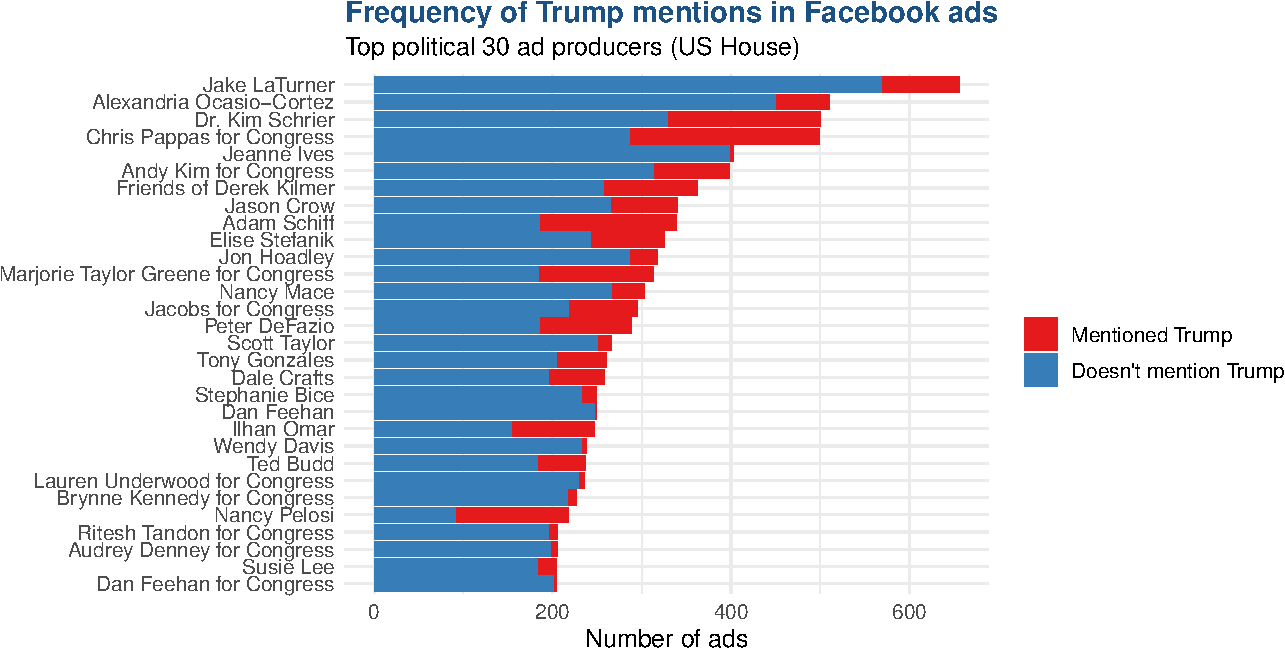
\includegraphics{figsFB/top30-trump-1.pdf}
\caption{\label{fig:top30-trump}Mentions of Trump}
\end{figure}

\begin{figure}
\centering
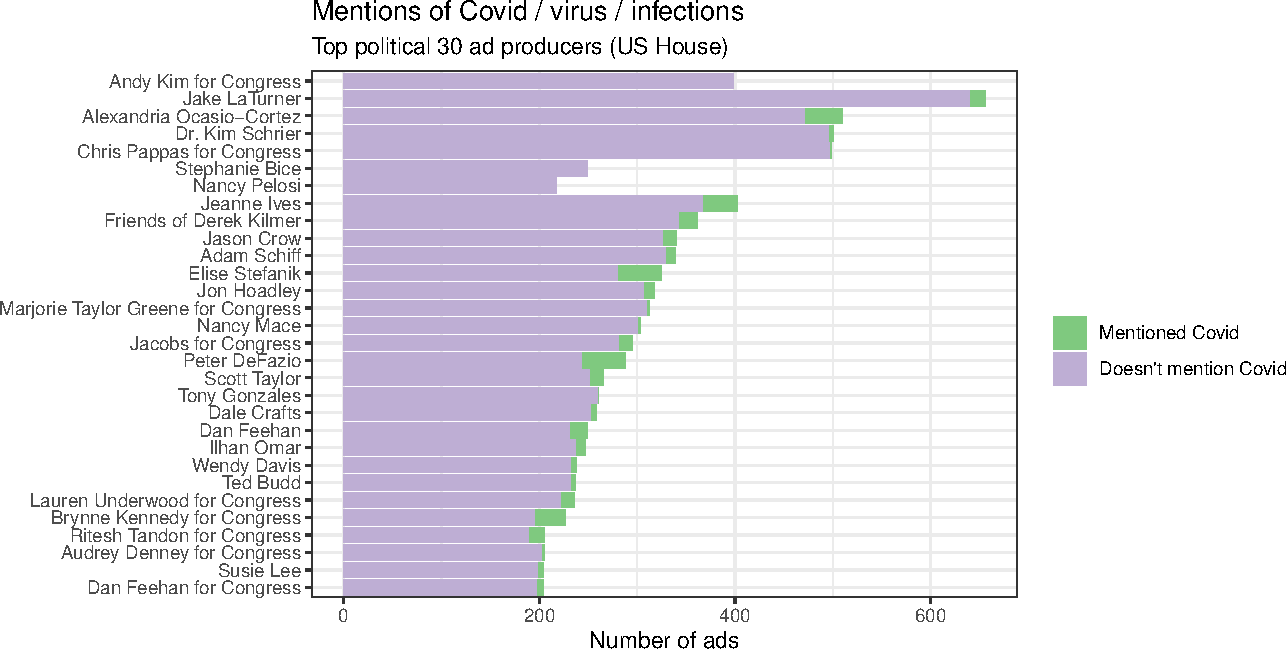
\includegraphics{figsFB/top30-covid-1.pdf}
\caption{\label{fig:top30-covid}Mentions of Covid}
\end{figure}

\pagebreak

\hypertarget{usage-of-salient-words-broken-down-by-pid}{%
\subsection{Usage of salient words, broken down by PID}\label{usage-of-salient-words-broken-down-by-pid}}

\begin{figure}
\centering
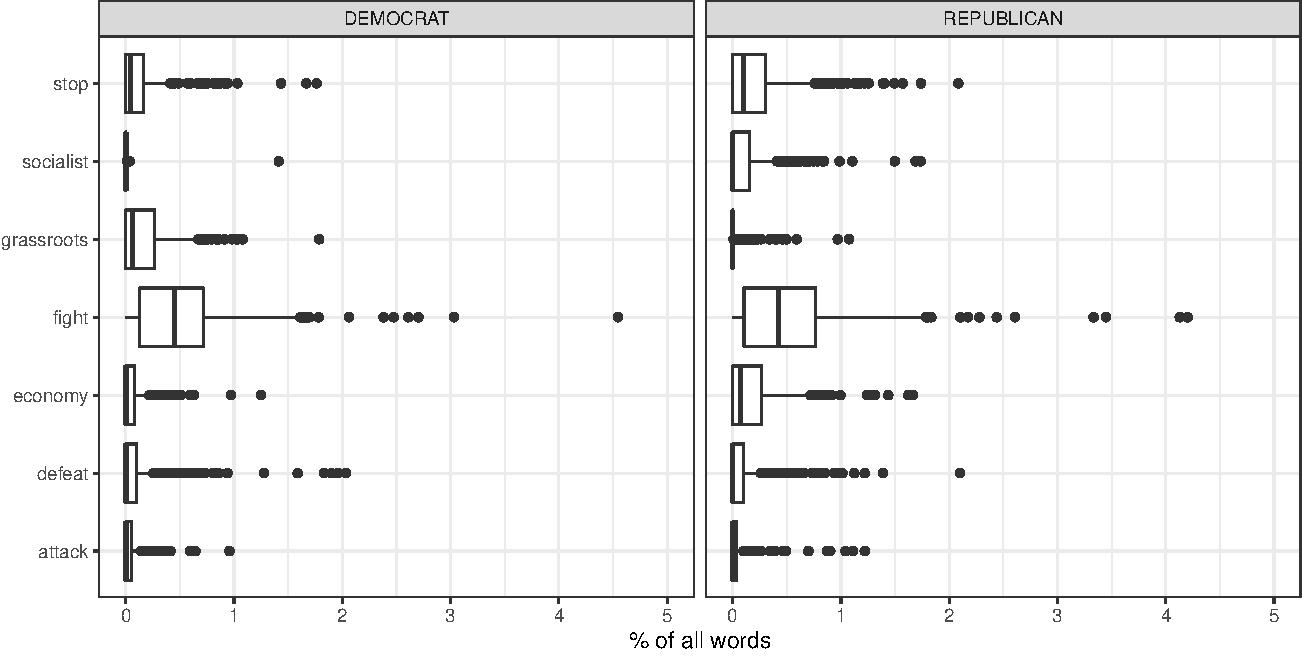
\includegraphics{figsFB/unnamed-chunk-3-1.pdf}
\caption{\label{fig:unnamed-chunk-3}Candidate-level usage of selected words (\% of all words used in ads)}
\end{figure}

\hypertarget{who-produced-most-words-for-fb-ads}{%
\subsection{Who produced most words for FB ads?}\label{who-produced-most-words-for-fb-ads}}

\begin{figure}
\centering
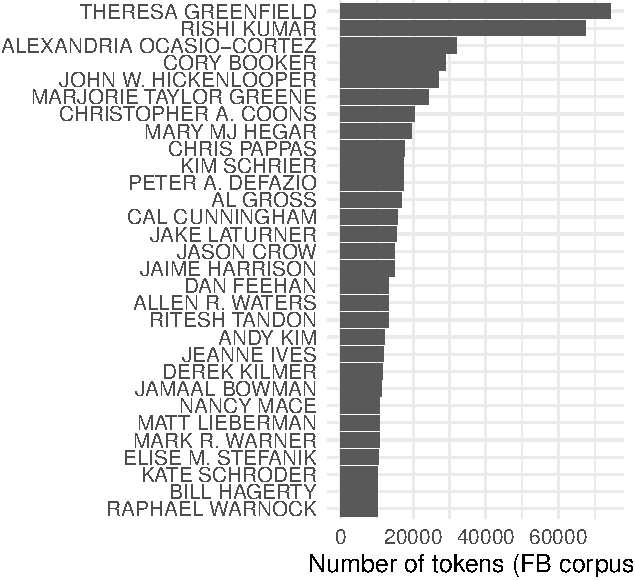
\includegraphics{figsFB/unnamed-chunk-4-1.pdf}
\caption{\label{fig:unnamed-chunk-4}Number of tokens by the 30 most prolific candidates}
\end{figure}

\pagebreak

\hypertarget{top-features-20-most-frequently-occurring-tokens}{%
\section{Top features (20 most frequently occurring tokens)}\label{top-features-20-most-frequently-occurring-tokens}}

\hypertarget{all-fb-ads}{%
\paragraph{All FB ads}\label{all-fb-ads}}

\begin{verbatim}
##      help       can         $       now        us      need  congress  campaign 
##     18198     15392     14848     13992     13590     13045     11491     10767 
##     today     trump     fight    senate      back   support    people      chip 
##     10538     10067      9586      9237      9006      8508      8446      7930 
##      vote president      make      join 
##      7789      7572      7329      7323
\end{verbatim}

\hypertarget{democrats}{%
\paragraph{Democrats}\label{democrats}}

\begin{verbatim}
##     help      can        $      now     need       us campaign    today 
##    12627    11707    10854    10318     9956     9879     8374     7064 
##   senate congress    fight     chip   people     back    trump     make 
##     6934     6887     6424     6250     6188     5711     5573     5520 
##     take     join     just  support 
##     4966     4787     4622     4613
\end{verbatim}

\hypertarget{republicans}{%
\paragraph{Republicans}\label{republicans}}

\begin{verbatim}
##         help    president     congress        trump            $      support 
##         5568         5077         4596         4494         3992         3889 
##           us          now          can        today         back         vote 
##         3677         3668         3659         3456         3291         3275 
##        fight         need conservative        stand         join    democrats 
##         3160         3084         2583         2579         2527         2418 
##         like     campaign 
##         2398         2389
\end{verbatim}

\hypertarget{dictionary-anlysis}{%
\section{Dictionary anlysis}\label{dictionary-anlysis}}

\hypertarget{trolling-words-by-ad-type}{%
\subsection{Trolling words by ad type}\label{trolling-words-by-ad-type}}

When a donation link is included, the language is on average more aggressive:

\begin{figure}
\centering
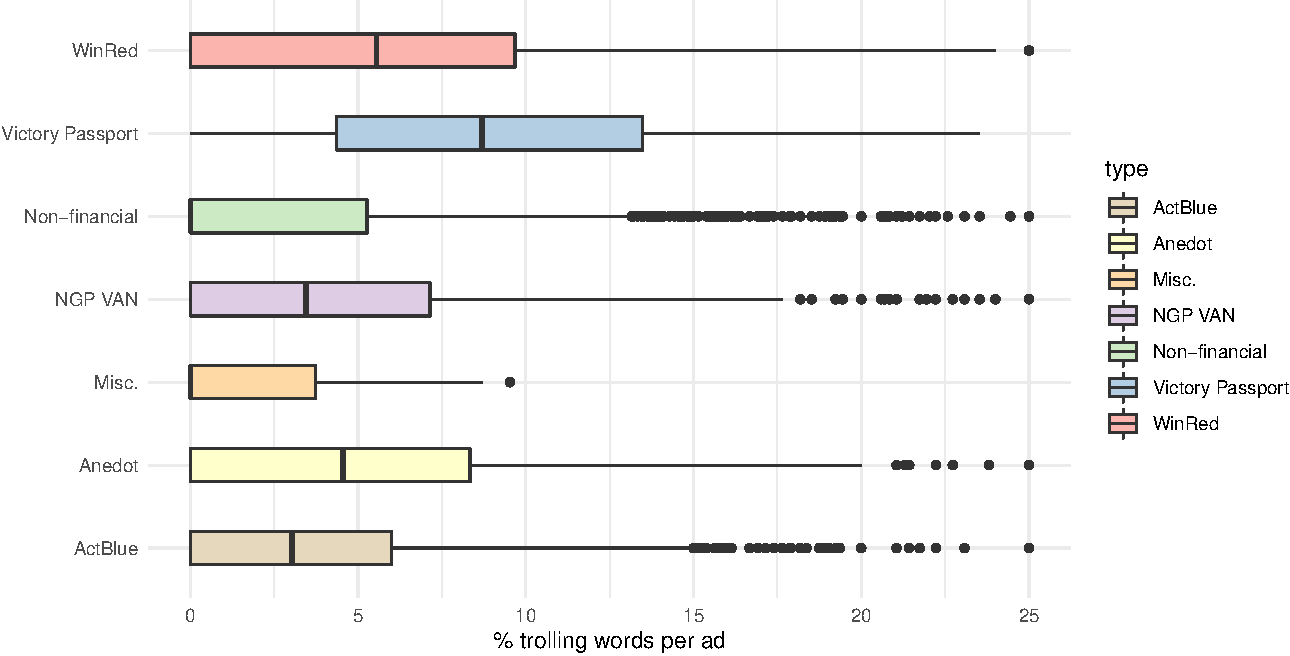
\includegraphics{figsFB/unnamed-chunk-10-1.pdf}
\caption{\label{fig:unnamed-chunk-10}Percent of trolling words per ad, broken down by ad type}
\end{figure}

\begin{figure}
\centering
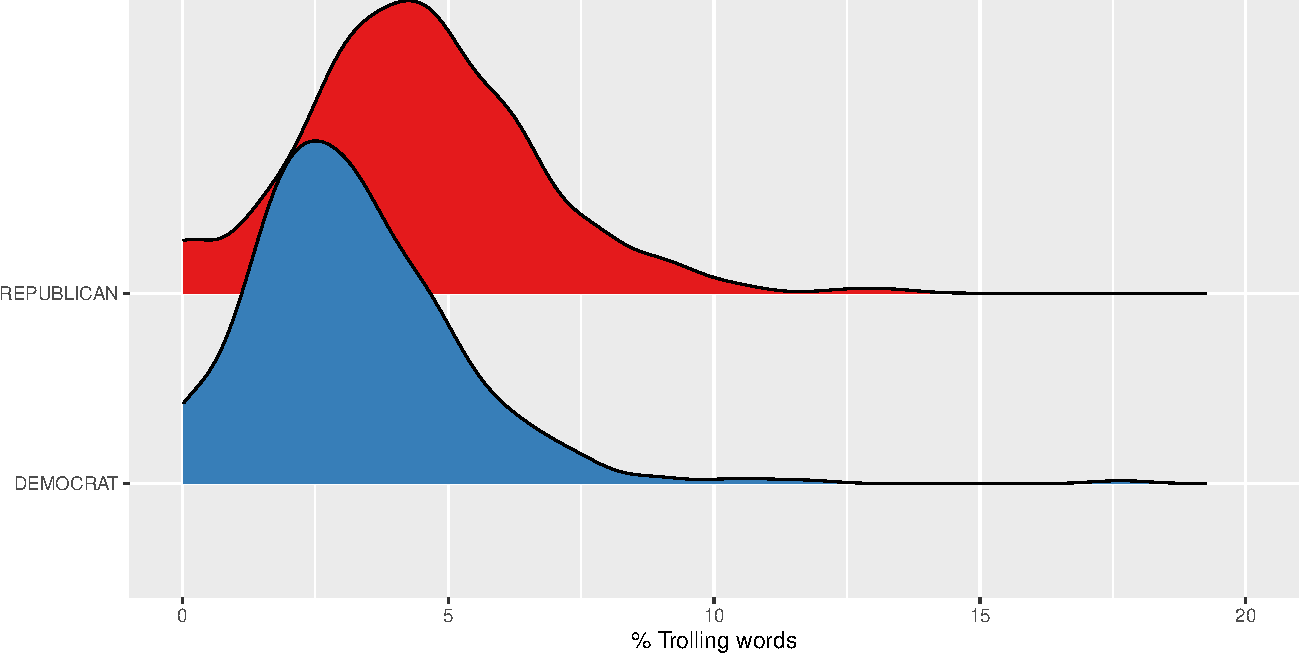
\includegraphics{figsFB/unnamed-chunk-11-1.pdf}
\caption{\label{fig:unnamed-chunk-11}Percent of trolling words per ad, broken down by ad type and by Party ID}
\end{figure}

\pagebreak
\clearpage

\hypertarget{trolling-words-candidate-level-analysis---proprtions}{%
\subsection{Trolling words {[}candidate-level analysis - PROPRTIONS{]}}\label{trolling-words-candidate-level-analysis---proprtions}}

\begin{figure}
\centering
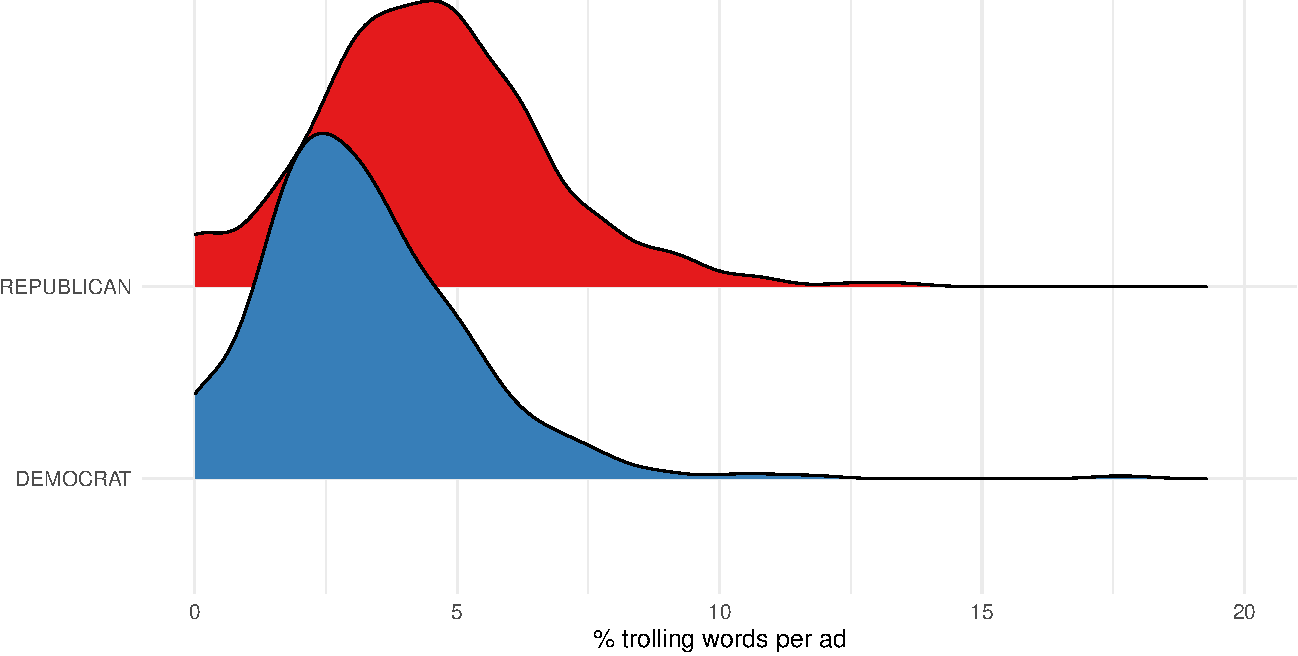
\includegraphics{figsFB/unnamed-chunk-12-1.pdf}
\caption{\label{fig:unnamed-chunk-12}Distribution of candidate-level average of trolling usage (broken down by Party ID)}
\end{figure}

\begin{figure}
\centering
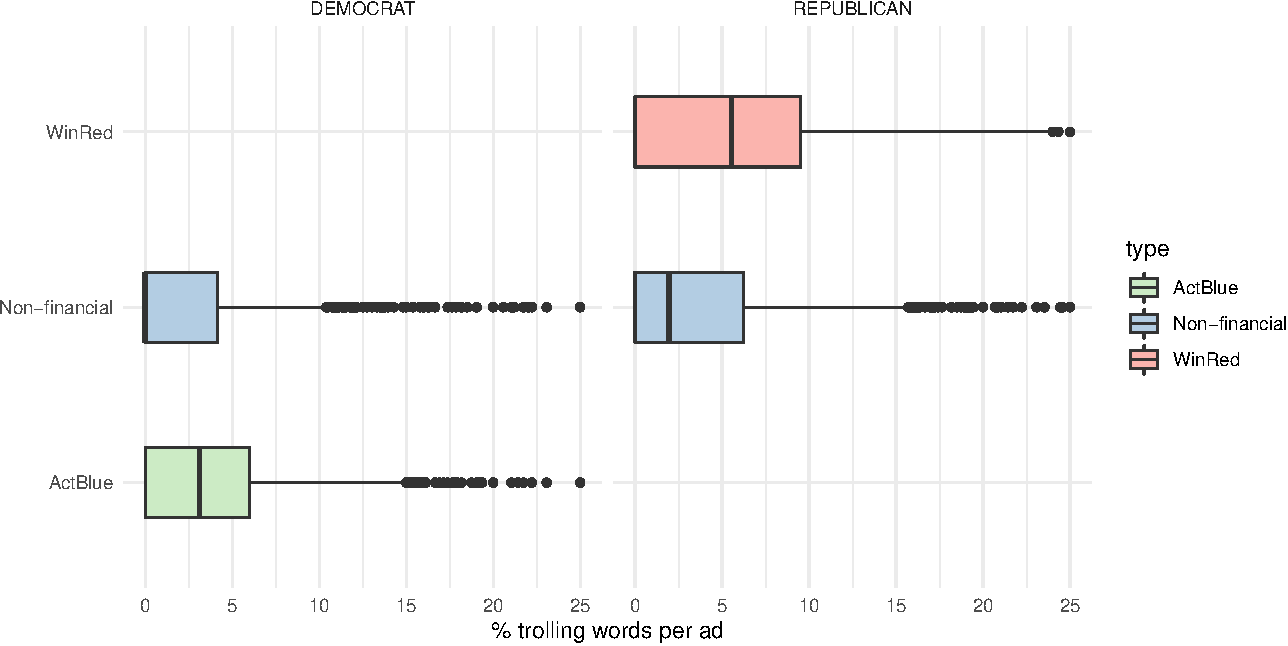
\includegraphics{figsFB/unnamed-chunk-13-1.pdf}
\caption{\label{fig:unnamed-chunk-13}Distribution of candidate-level average of trolling usage (broken down by Party ID and chamber of Congress)}
\end{figure}

\begin{figure}
\centering
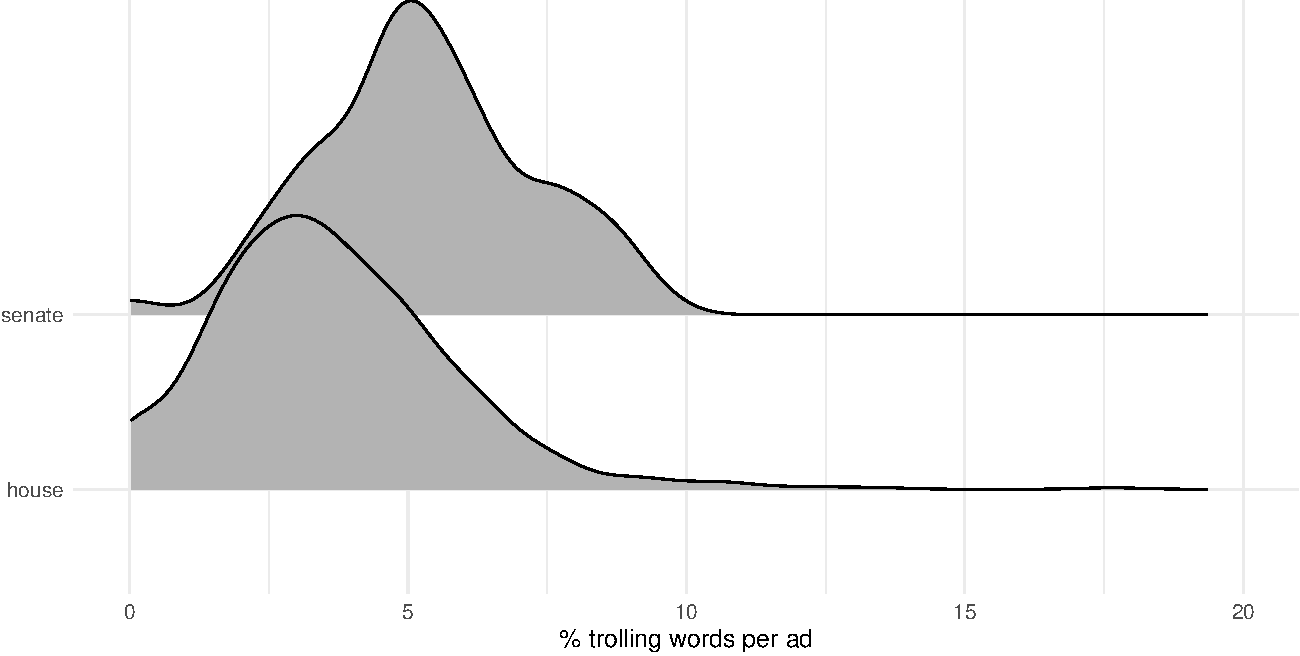
\includegraphics{figsFB/unnamed-chunk-14-1.pdf}
\caption{\label{fig:unnamed-chunk-14}Candidate-level average usage of trolling words, broken down by chamber}
\end{figure}

\pagebreak
\clearpage

\hypertarget{trolling-words-ad-level-analysis}{%
\subsection{Trolling words {[}ad-level analysis{]}}\label{trolling-words-ad-level-analysis}}

\begin{figure}
\centering
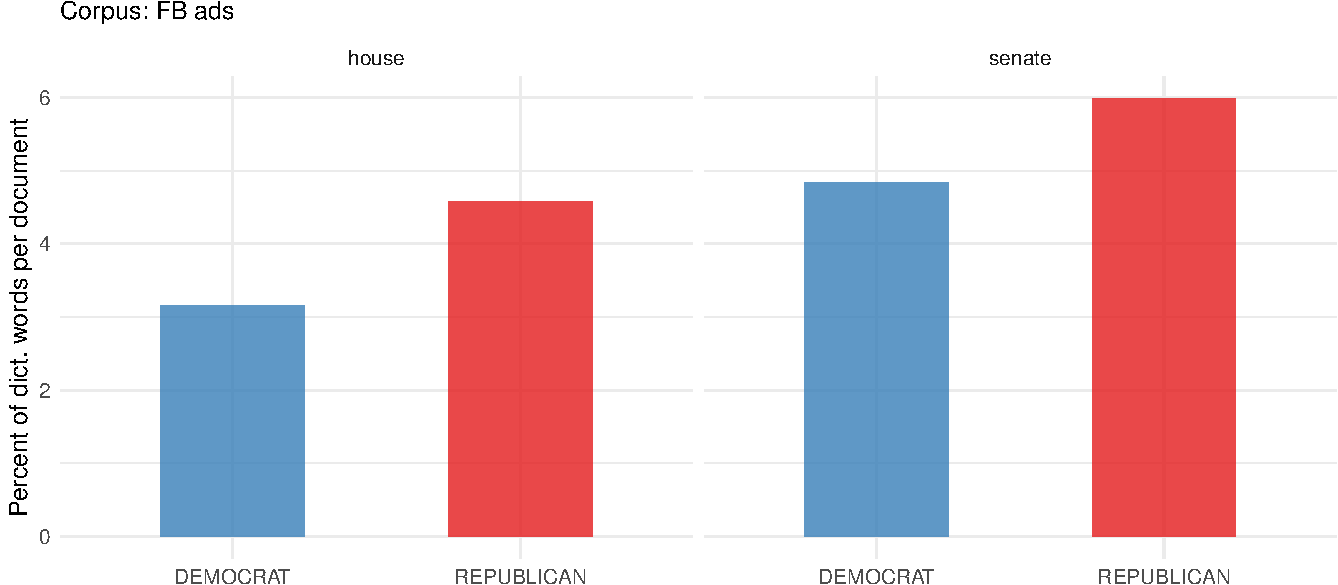
\includegraphics{figsFB/unnamed-chunk-15-1.pdf}
\caption{\label{fig:unnamed-chunk-15}Average proportion of trolling words per ad, broken down by party ID and chamber}
\end{figure}

\begin{figure}
\centering
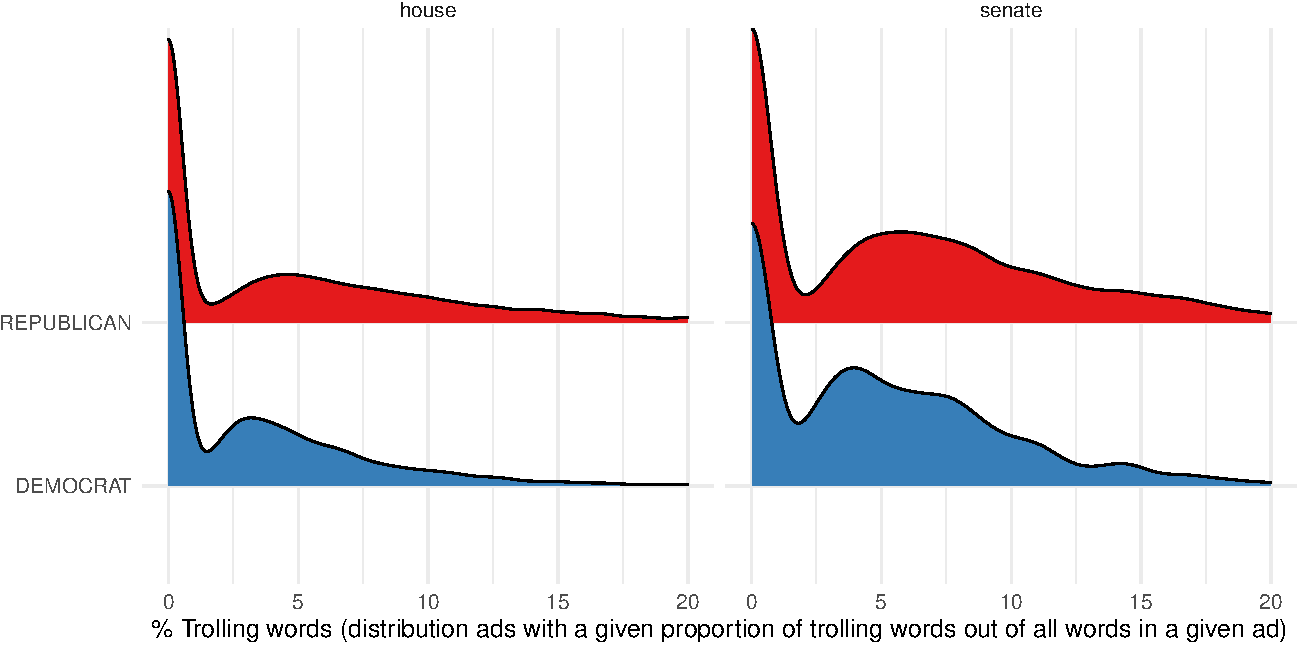
\includegraphics{figsFB/unnamed-chunk-16-1.pdf}
\caption{\label{fig:unnamed-chunk-16}Distribution of trolling words per ad, broken down by party ID and chamber}
\end{figure}

\pagebreak
\clearpage

\hypertarget{trolling-words-ad-level-analysis---counts}{%
\subsection{Trolling words {[}ad-level analysis - COUNTS{]}}\label{trolling-words-ad-level-analysis---counts}}

\begin{figure}
\centering
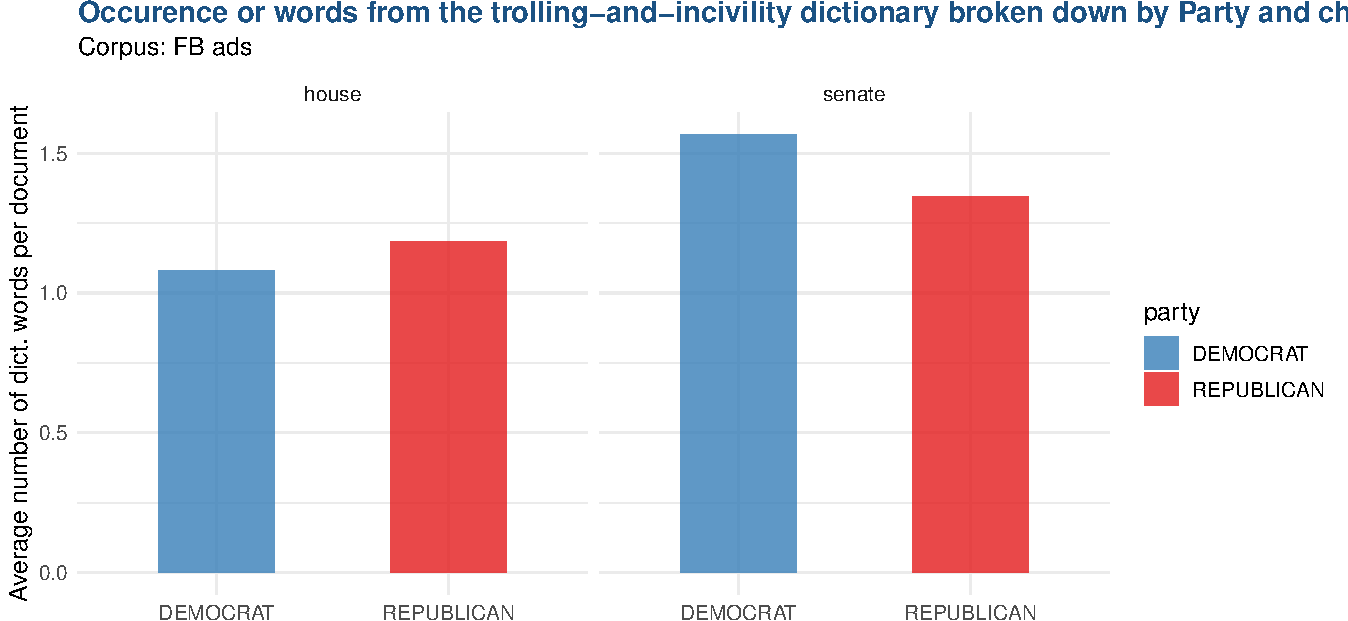
\includegraphics{figsFB/unnamed-chunk-17-1.pdf}
\caption{\label{fig:unnamed-chunk-17}Average number of trolling words by party and chamber}
\end{figure}

\pagebreak
\clearpage

\hypertarget{trolling-words-candidate-level-analysis---counts}{%
\subsection{Trolling words {[}candidate-level analysis - COUNTS{]}}\label{trolling-words-candidate-level-analysis---counts}}

\begin{figure}
\centering
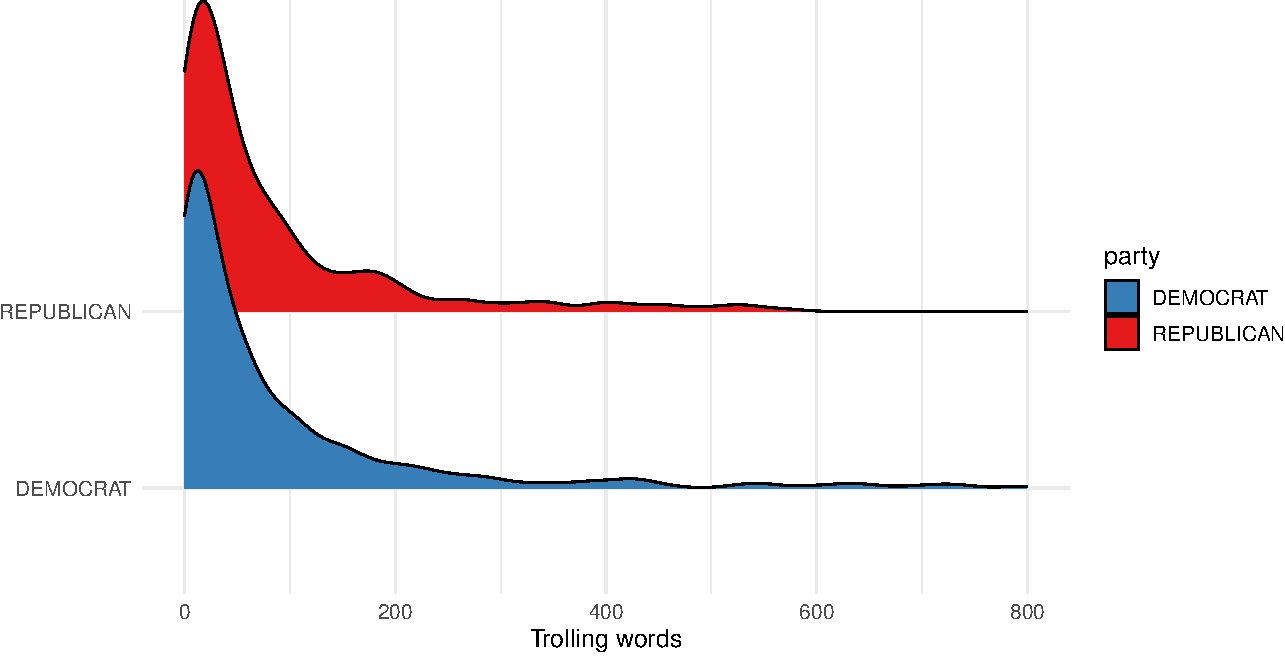
\includegraphics{figsFB/unnamed-chunk-18-1.pdf}
\caption{\label{fig:unnamed-chunk-18}Distribtion of candidate-level trolling words counts (totals)}
\end{figure}

\begin{figure}
\centering
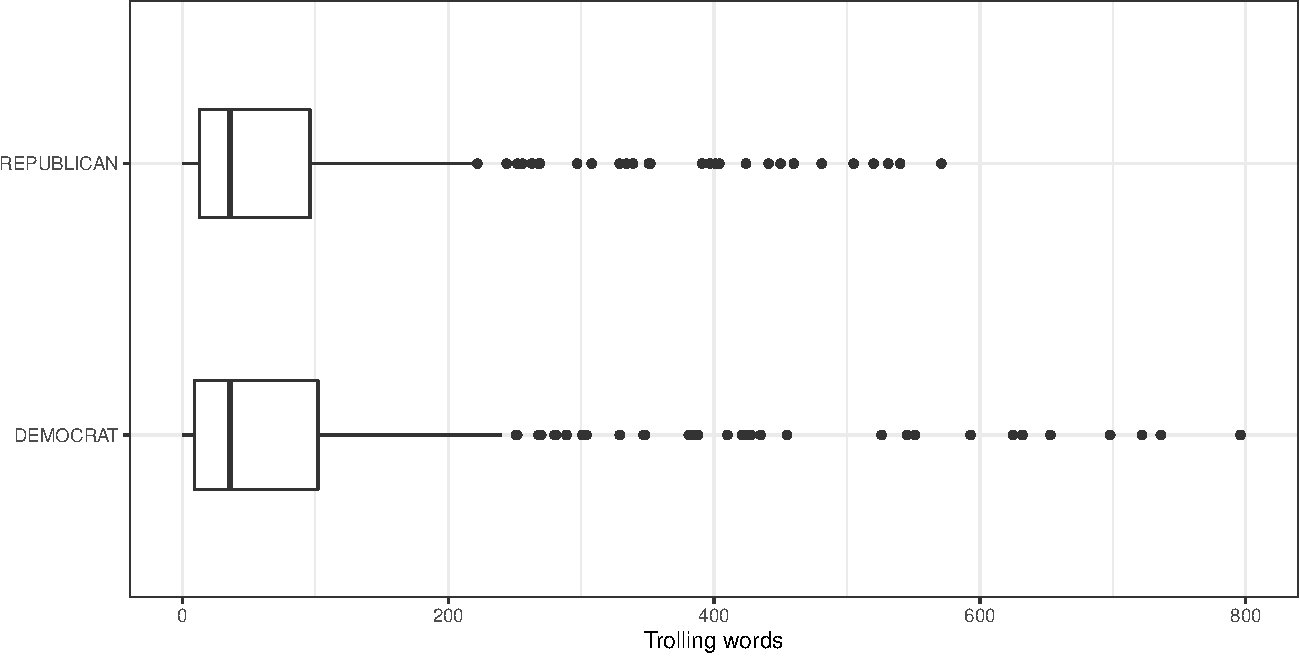
\includegraphics{figsFB/unnamed-chunk-19-1.pdf}
\caption{\label{fig:unnamed-chunk-19}Distribtion of candidate-level trolling words counts (totals)}
\end{figure}

\begin{figure}
\centering
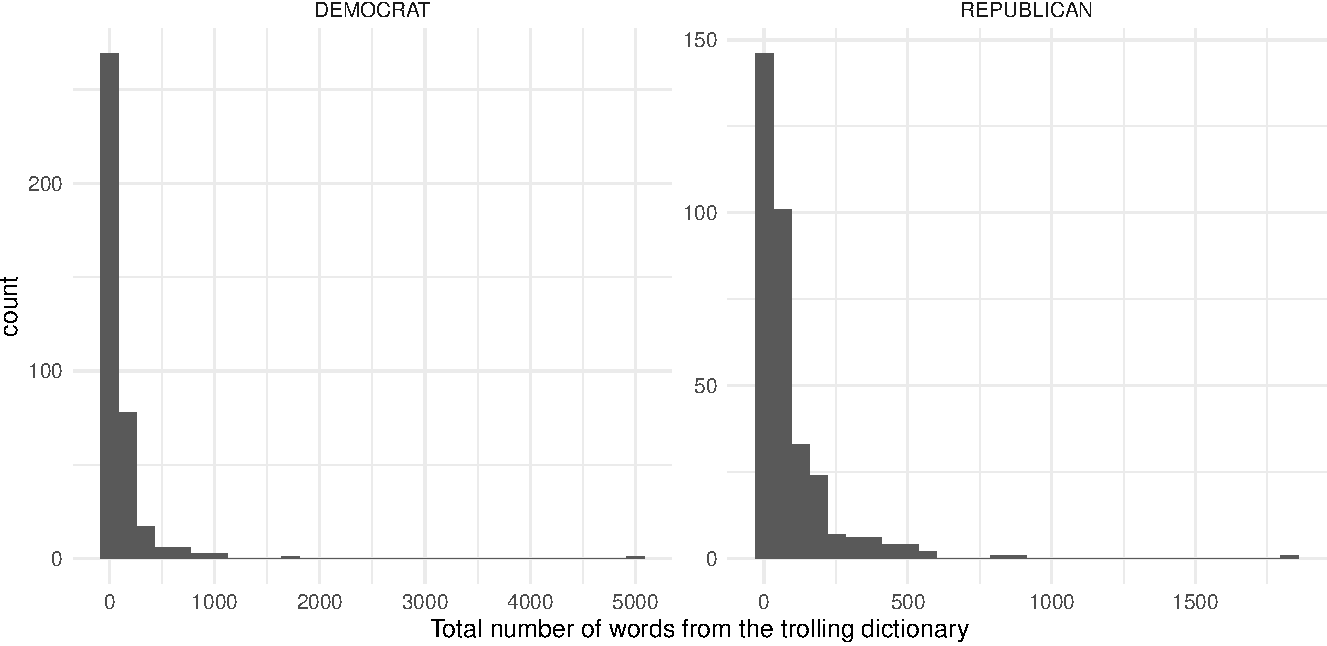
\includegraphics{figsFB/unnamed-chunk-20-1.pdf}
\caption{\label{fig:unnamed-chunk-20}Total number of trolling words in the corpus produced by candidates}
\end{figure}

\clearpage
\pagebreak

\hypertarget{moral-foundations-candidate-level-analysis}{%
\subsection{Moral foundations {[}candidate-level analysis{]}}\label{moral-foundations-candidate-level-analysis}}

\begin{figure}
\centering
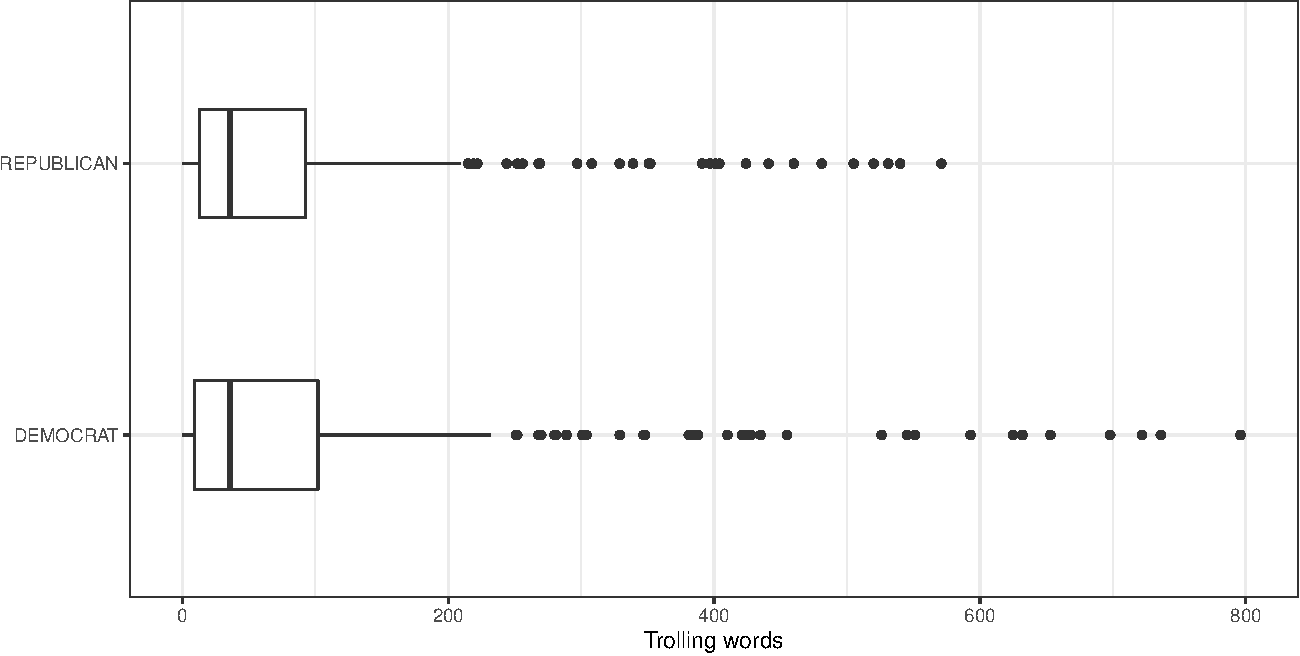
\includegraphics{figsFB/unnamed-chunk-21-1.pdf}
\caption{\label{fig:unnamed-chunk-21}Distribution of Moral foundations words in FB ads, by party}
\end{figure}

\begin{figure}
\centering
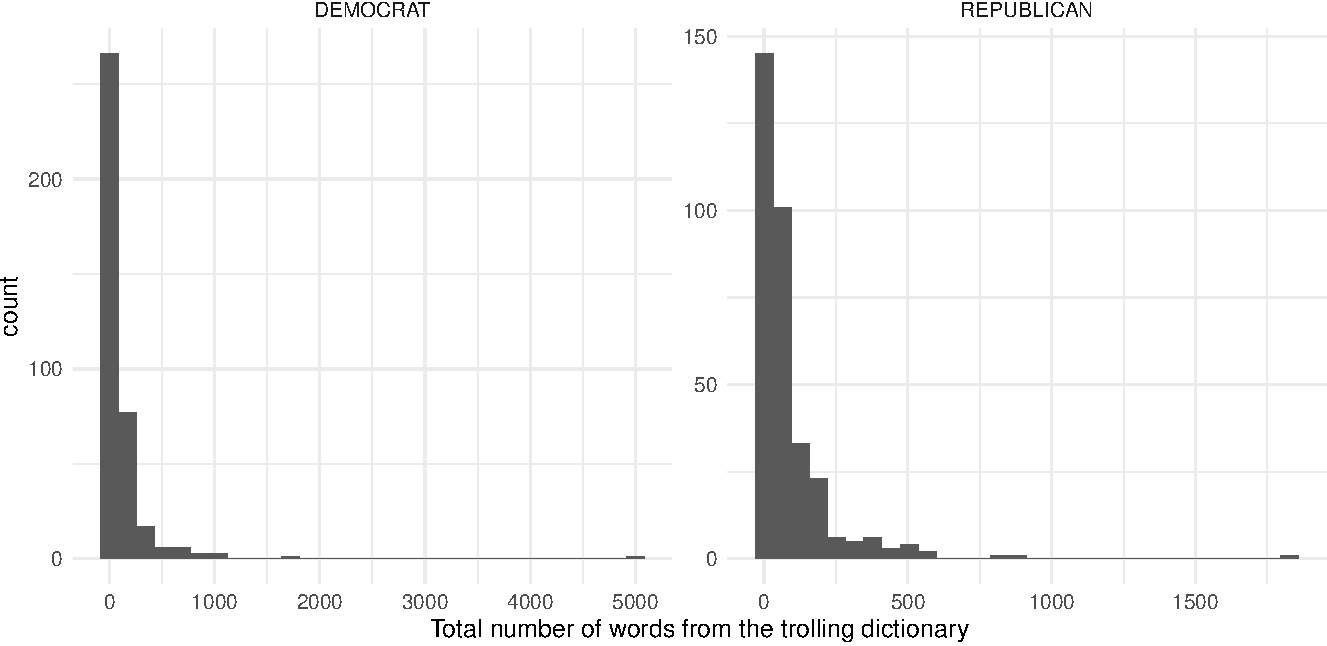
\includegraphics{figsFB/unnamed-chunk-22-1.pdf}
\caption{\label{fig:unnamed-chunk-22}Candidate-level usage of moral words (MFD)}
\end{figure}

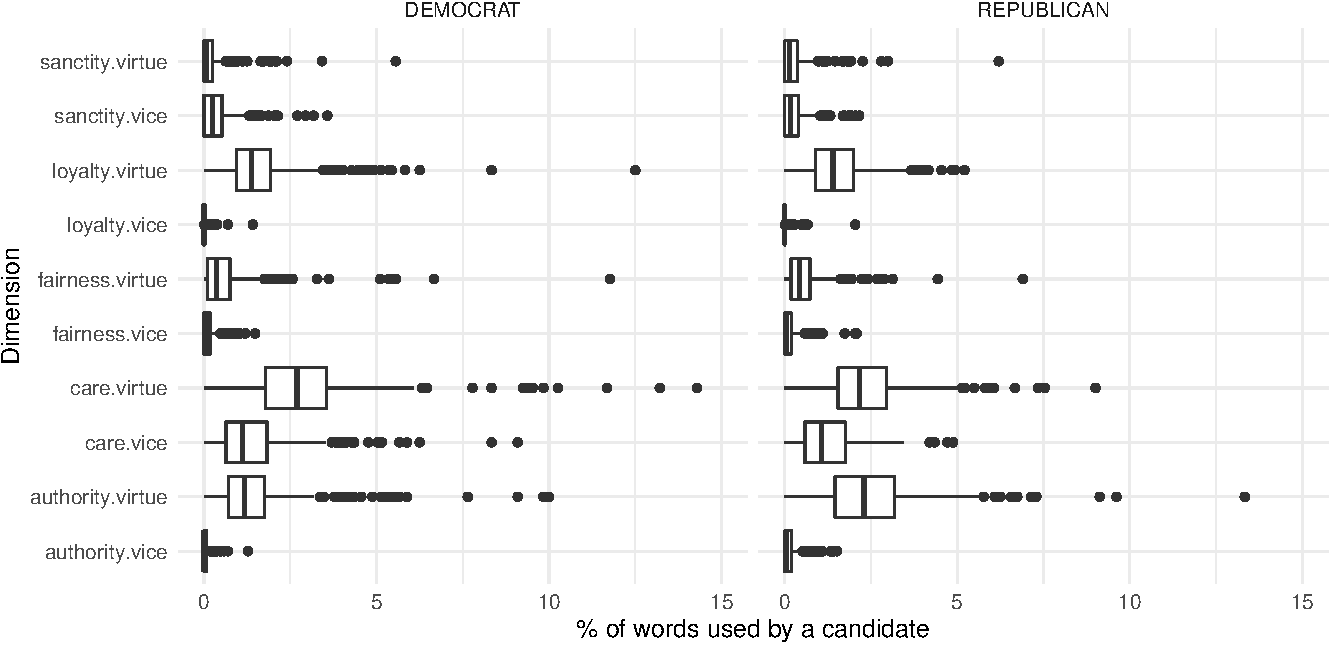
\includegraphics{figsFB/Candidate-level usage of moral words (MFD)-1.pdf}

\begin{table}

\caption{\label{tab:unnamed-chunk-23}Average Usage of words across candidates, broken down by Party ID}
\centering
\begin{tabular}[t]{lrr}
\toprule
Average Usage of the dimension Per Candidate (in \%) & DEMOCRAT & REPUBLICAN\\
\midrule
authority.vice & 0.06 & 0.16\\
authority.virtue & 1.41 & 2.53\\
care.vice & 1.37 & 1.22\\
care.virtue & 2.93 & 2.33\\
fairness.vice & 0.13 & 0.14\\
\addlinespace
fairness.virtue & 0.65 & 0.56\\
loyalty.vice & 0.01 & 0.03\\
loyalty.virtue & 1.57 & 1.54\\
sanctity.vice & 0.38 & 0.27\\
sanctity.virtue & 0.24 & 0.30\\
\bottomrule
\end{tabular}
\end{table}

\end{document}
